\subsection{Ondas}

\begin{multicols}{2}
  Este filtro combina la imagen original con una imagen de ondas, dando tonos más oscuros y mas claros en forma de onda. Estas se centran en un punto de la imagen -pasado como parámetro- y se expanden hacia sus bordes de manera concéntrica. Para ello aplicamos implementamos el pseudocódigo del algoritmo otorgado por la cátedra, en el cual a cada pixel de la imagen se le suma un valor de profundidad basado en su distancia al centro de las ondas.
  \begin{center}
    \begin{tabular}{cccc}
      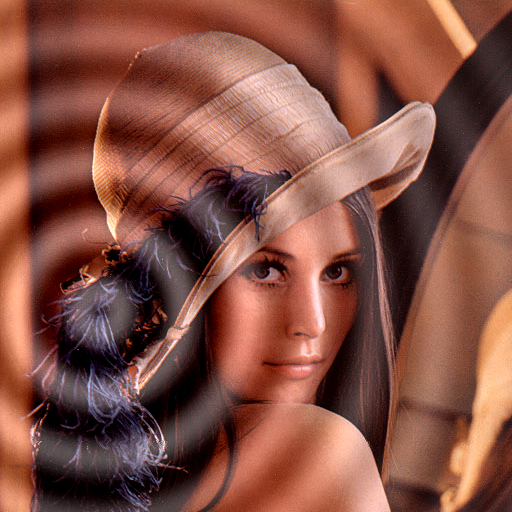
\includegraphics[width=0.3\textwidth]{imagenes/lenaONDA.jpg} \\
    \end{tabular}
     \end{center}
  \end{multicols}

\subsubsection{Implementación C}

Nuestra implementación en C es una traducción iterativa del mencionado algoritmo propuesto por la cátedra en el siguiente pseudocódigo:

\begin{algorithm}[H]
  \begin{algorithmic}[1]
    \FORALL{pixel ubicado en la posici'on $\mathbf{(x, y)}$}
      \STATE $d_x \gets x - x_0$
      \STATE
      \STATE $d_y \gets y - y_0$
      \STATE
      \STATE $d_{xy} \gets \sqrt{d_{x}^2+d_{y}^2}$
      \STATE
      \STATE $r \gets \frac{(d_{xy} - RADIUS)}{WAVELENGTH}$
      \STATE
      \STATE $a \gets \frac{1}{1 + (\frac{r}{TRAINWIDTH})^2 }$
      \STATE
      \STATE $t \gets ( r-floor(r) ) \cdot 2 \cdot \pi - \pi$
      \STATE
      \STATE $prof \gets a \cdot (t - \frac{t^3}{6}+\frac{t^5}{120}-\frac{t^7}{5040})$
      \STATE
      \STATE $pixel = prof \cdot 64 + I_{src}(x, y)$    
      \STATE
      \STATE $I_{dst}(x, y) = saturar(pixel)$
    \ENDFOR
  \end{algorithmic}
  \caption{$ondas (I_{src}, I_{dst}, x_0, y_0)$}
  \label{alg:ondas}
\end{algorithm}

\begin{itemize}
  \item $x_0$ e $y_0$ representan la posici'on donde est'a centrada la onda,
  \item $RADIUS$, $WAVELENGTH$ y $TRAINWIDTH$ son constantes que definen la 
  forma de la onda y
  \item $saturar(x)$ es una funci'on que retorna $0$ si $x$ es menor $0$, $255$
  si es mayor a $255$ y $x$ en cualquier otro caso.
\end{itemize}

\subsubsection{Implementación ASM}
Es este ejercicio procesaremos de a 4 píxeles, por cada iteracion sobre la imagen.
\subsubsection*{Cálculo de la profudidad}
Vamos a dar una breve explicación del cáculo de la profundidad en assembler.

\subsubsection*{caculo de la distancia}

Est este ejecicio queremos calcular la distancia, esto es $\sqrt{(x-x_0)^2+(y-y_0)^2} = \sqrt{dx^2+dy^2}$.
Este proceso lo hacemos con los 4 píxeles juntos.
La idea es obtener en \emph{xmm3=$|(dx3^2+dy3^2)^{1/2}|$...$|(dx0^2+dy0^2)^{1/2}|$}. Podemos observar abajo el detalle de cada calculo e instrucción usada.
\begin{codesnippet}
\begin{verbatim}
                            ;CALCULO DE PROFUNDIDAD
                            ;xmm11=|x_0|x_0|x_0|x_0| Centro de la onda eje x
                            :xmm14=|y_0|y_0|y_0|y_0| Centro de la onda eje y
    movdqu xmm3, xmm11      ;xmm3=|x3|x2|x1|x0| 
    psubd xmm3, xmm13       ;xmm3=|x3-x_0|x2-x_0|x1-x0|x0-x_0|                    x - x_0
							
    movdqu xmm4, xmm12      ;xmm4=|y1|y2|y3|y4|
    psubd xmm4, xmm14       ;xmm4=|y3-y_0|y2-y_0|y1-y_0|y0-y_0|                     y - y_0	
                            ;sabiendo dx3=x3-x_0,dx2=x2-x_0,dx1=x1-x_0 y dx0=x0-x_0
    pmulld xmm3, xmm3       ;xmm3=|dx3^2|dx2^2|dx1^2|dx0^2|
    pmulld xmm4, xmm4       ;xmm4=|dy3^2|dy2^2|dy1^2|dy0^2|
                            ;Realizamos la suma dx^2+dy^2
    paddd xmm3, xmm4        ;xmm3=|dx3^2+dy3^2|...|dx0^2+dy0^2|
                            ; Convertimos de doble word integer a Float
    cvtdq2ps xmm3, xmm3     ;xmm3= Convertimos de doble word integer a Float
                            ;Sacamos raiz cuadrada a cada paquet dobleWord, o sea (dx^2+dy^2)^(1/2)
    sqrtps xmm3, xmm3       ;xmm3=|(dx3^2+dy3^2)^(1/2)|...|(dx0^2+dy0^2)^(1/2)|
\end{verbatim}
\end{codesnippet}


\subsubsection*{Cálculos auxiliares(variables R, K, A y T)}

En esta sección queremos cálcular:

\begin{center}
	$R \gets (dxy-RADIUS)/WAVELENGTH$\\
	$K \gets R-floor(r)$ \\
	$A \gets \frac{1.0}{(1.0+(\frac{r}{TRAINWIDTH)}*\frac{r}{TRAINWIDTH))}}$ \\
	$T \gets K*2*PI-PI$
\end{center}

\begin{codesnippet}
\begin{verbatim}
                                ;Calculo de R, o sea (dx*dx+dy*dy)^(1/2) - RADIO 
                                ;xmm9=|RADIO|RADIO|RADIO|RADIO|
    subps xmm3, xmm9            ;xmm3=|dxy3-RADIO|dxy2-RADIO|dxy1-RADIO|dxy0-RADIO| donde dxy es la distancia
                                ;xmm8=|WAVELENGTH|WAVELENGTH|WAVELENGTH|WAVELENGTH|
                                ; R <- ((dx*dx+dy*dy)^(1/2) - RADIO)/WAVELENGTH
    divps xmm3, xmm8            ;xmm3=|R3|R2|R1|R0|	
;###################################################################################
                                ;Calculo de K
    movdqu xmm7, xmm3           ;xmm7=|R3|R2|R1|R0|
    movdqu xmm4, xmm3           ;xmm4=|R3|R2|R1|R0|
                                ;El valor 0001b me permite activar la opcion de TRUNCAR c/u Float
                                ;Donde floor(R) es el el truncamiento
    roundps xmm3, xmm3, 0001b   ;xmm3=|floor(R3)|floor(R2)|floor(R1)|floor(R0)|

                                ;K  <- R - floor(R)
    subps xmm4, xmm3            ;xmm4=|R3-floor(R3)|R2-floor(R2)|R1-floor(R1)|R0-floor(R0)|								
                                ;xmm4=|k3|k2|k1|k0|
                                ;xmm3 <- R
                                ;xmm4 <- K
;######################################################################################
                                ;Cálculo de T
    movdqu xmm5, xmm4           ;xmm5=|k3|k2|k1|k0|
                                ;xmm10=|1|1|1|1| 
    paddd xmm10, xmm10          ;xmm10=|2|2|2|2|
    cvtdq2ps xmm10, xmm10       ;xmm10=|2|2|2|2| convierto a Floats
    mulps xmm5, xmm10           ;xmm5=|k3*2|k2*2|k1*2|k0*2| multiplico por 2 a los k's
    divps xmm10, xmm10          ;xmm10=|1.0|1.0|1.0|1.0| floats
    cvtps2dq xmm10, xmm10       ;xmm10=|1|1|1|1| convertimos de floats a integer
                                ;xmm6=|PI|PI|PI|PI|
    mulps xmm5, xmm6            ;xmm5=|k3*2*PI|k2*2*PI|k1*2*PI|k0*2*PI|
                                ;Queremos realizar lo siguiente  t = k*2*PI-PI
    subps xmm5, xmm6            ;xmm5=|k3*2*PI-PI|k2*2*PI-PI|k1*2*PI-PI|k0*2*PI-PI|
                                ;xmm5=|T3|T2|T1|T0| donde T=k*2*PI-PI 
;######################################################################################
                                ;Calculo de A
    movdqu xmm3, xmm7           ;xmm3=|R3|R2|R1|R0|
                                ;R/TRAINDIWTH
    divps xmm3, xmm15           ;xmm3=|R3/TRAINDIWTH|R2/TRAINDIWTH|R1/TRAINDIWTH|R0/TRAINDIWTH|
                                ;R/TRAINDIWTH * R/TRAINDIWTH
    mulps xmm3, xmm3            ;xmm3=|(R3/TRAINDIWTH)^2|...|(R0/TRAINDIWTH)^2|
    cvtdq2ps xmm10, xmm10       ;xmm10=|1.0|1.0|1.0|1.0| convertimos de Integer a Floats
                                ;1 + (R/TRAINDIWTH * R/TRAINDIWTH)
    addps xmm3, xmm10           ;xmm3=|1 + (R1/TRAINDIWTH)^2|...|1 + (R0/TRAINDIWTH)^2|
    movdqu xmm4, xmm10          ;xmm4= |1.0|1.0|1.0|1.0|
                                ;A = 1 / 1 + (R/TRAINDIWTH * R/TRAINDIWTH)
    divps xmm4, xmm3            ;xmm4=|A3|A2|A1|A0|
\end{verbatim}
\end{codesnippet}

\subsubsection*{Cálculos Sin_Taylor}
En esta parte queremos hacer el cálculos de
\begin{center}
	$SinTaylor \gets (t - \frac{t^3}{6}+\frac{t^5}{120}-\frac{t^7}{5040})$ \\
	$prof \gets A * SinTaylor*64$
\end{center}
Veremos q en $xmm4=|A3*(t3-t3^3/6+t3^5/120-t3^7/5040)*64|...|A1*(t0-t0^3/6+t0^5/120-t0^7/5040)*64|$ el Sin Taylor Buscado.
\begin{codesnippet}
\begin{verbatim}
                            ;sin taylor
    movdqu xmm1, xmm5       ;xmm1=|t3|t2|t1|t0|
                            ;calculamos x al cubo
    movdqu xmm3, xmm5       ;xmm3=|t3|t2|t1|t0|
    mulps xmm3, xmm5        ;xmm3=|t3^2|t2^2|t1^2|t0^2|
    mulps xmm3, xmm5        ;xmm3=|t3^3|t2^3|t1^3|t0^3|	

    movq xmm2, r15          ;xmm2=|0|0|0|6|
    packssdw xmm2, xmm2     ;xmm2=|0|6|0|6|
    packssdw xmm2, xmm2     ;xmm2=|6|6|6|6|
    cvtdq2ps xmm2, xmm2	    ;xmm2=|6|6|6|6| convierto de integer a Floats

    divps xmm3, xmm2        ;xmm3=|(t3^3)/6|(t2^3)/|(t1^3)/6|(t0^3)/6|
    subps xmm1, xmm3        ;xmm1=|t3-(t3^3)/6|t2-(t2^3)/|t1-(t1^3)/6|t0-(t0^3)/6|
                     ...............                  
                            ;Calculamos T a la quinta
                            ;Los calculos son analogos y obtenemos los siguiente
                     ...............
    divps xmm3, xmm2        ;xmm3=|t3^5/120|t2^5/120|t1^5/120|t0^5/120|								
    addps xmm1, xmm3        ;xmm1=|t3-(t3^3)/6+t3^5/120|...|t0-(t0^3)/6+t0^5/120|								
                     ................... 
                            ;Cálculamos T a la septima
                            ;Cálculos analogos
                    ................	
    divps xmm3, xmm2        ;xmm3=|t3^7/5040|t2^7/5040|t1^7/5040|t0^7/5040|
                    
    subps xmm1, xmm3        ;xmm1=|t3-(t3^3)/6+t3^5/120-t3^7/5040|...|t0-(t0^3)/6+t0^5/120-t0^7/5040|

    subps xmm1, xmm3        ;xmm1=|t3-(t3^3)/6+t3^5/120-t3^7/5040|...|t0-(t0^3)/6+t0^5/120-t0^7/5040|								
                    ................
                            ;Cálculamos la multiplicacion por A y por 64
    mulps xmm4, xmm1        ;xmm4=|A3*(t3-t3^3/6+t3^5/120-t3^7/5040)|...|A1*(t0-t0^3/6+t0^5/120-t0^7/5040(|
                            ;Renombramos a xmm4=|prof3|prof2|prof1|prof0|		
    mulps xmm4, xmm8        ;xmm4=|prof3*64|prof2*64|prof1*64|prof0*64|

\end{verbatim}
\end{codesnippet}

\subsubsection*{Agregar profundidad a los pixeles(ultímo paso)}
En este paso ya tenemos el cálculo de la profundidad en el registro $xmm4$, sólamente nos resta agregar la profundidad a los 4 pixeles q estamos por procesar. O sea falta lo siguinte:
\begin{center}
       $pixel \gets prof + I_{src}(x, y)$    
      
      $I_{dst}(x, y) \gets saturar(pixel)$
\end{center}
Abajo muestramos los segmentos mas importantes del codigo que lo resuelve.
\begin{codesnippet}
\begin{verbatim}
    cvtps2dq xmm4, xmm4             ;xmm4=|prof3*64|prof2*64|prof1*64|prof0*64| conviertimos de float a Integer

    movdqu xmm7, xmm4               ;xmm7=|prof3*64|prof2*64|prof1*64|prof0*64|
                                    ;me quedo con el 3er dobleWord usando el shuffle
    pshufd xmm4, xmm4, 11111111b    ;xmm4=|prof3*64|prof3*64|prof3*64|prof3*64|

    pxor xmm3, xmm3
                                    ;Levanto imagen en Xmm1
    movdqu xmm1, [rdi]              ;xmm1=|a3 b3 g3 r3|a2 b2 g2 r2|a1 b1 g1 r1|a0 b0 g0 r0|			
    movdqu xmm0, xmm1               ;xmm0=|a3 b3 g3 r3|a2 b2 g2 r2|a1 b1 g1 r1|a0 b0 g0 r0|
    punpckhbw xmm1, xmm3            ;xmm1=|a3 b3 g3 r3|a2 b2 g2 r2| de byte a word parte alta
    movdqu xmm2, xmm1               ;xmm2=|a3 b3 g3 r3|a2 b2 g2 r2| 
    punpckhwd xmm1, xmm3            ;xmm1=|a3 b3 g3 r3| de word a DobleWord parte alta
    punpcklwd xmm2, xmm3            ;xmm2=|a2 b2 g2 r2| de word a DobleWord parte baja
    paddd xmm1, xmm4                ;xmm1=|prof3*64+a3|prof3*64+b3|prof3*64+g3|prof3*64+r3|
                                    ;Renombro O(a3)=prof3*64+a3, etc
                                    ;xmm1=|O(a3) O(b3) O(g3) O(r3)|
#######################################################
    
    
                                    ; De Manera similar obtenmos xmm2
                                ......................			
    paddd xmm2, xmm4                ;xmm2=|a2+prof2*64|b2+prof2*64|g2+prof2*64|r2+prof2*64|
                                    ;xmm2=|O(a2)|O(b2)|O(g2)|O(r2)|	
                                    ;Empaquetamos de DobleWord a Word	
    packssdw xmm2,xmm1              ;xmm2=|O(a3) O(b3) O(g3) O(r3)|O(a2) O(b2) O(g2) O(r2)|
    movdqu xmm5, xmm2               ;xmm5=|O(a3) O(b3) O(g3) O(r3)|O(a2) O(b2) O(g2) O(r2)|
						.....................
    paddd xmm1, xmm4                ;xmm1=|a1+prof1*64|b1+prof1*64|g1+prof1*64|r1+prof1*64|
                                    ;xmm1=|O(a1)|O(b1)|O(g1)|O(r1)|						
                        .....................
    paddd xmm2, xmm4                ;xmm2=|a0+prof0*64|b0+prof0*64|g0+prof0*64|r0+prof0*64| shuffle posicion 0 de dobleWord
                                    ;xmm2=|O(a0)|O(b0)|O(g0)|O(r0)|                   
                                    ;Empaquetamos de DobleWord a Word
    packssdw xmm2,xmm1              ;xmm2=|O(a1) O(b1) O(g1) O(r1)|O(a0) O(b0) O(g0) O(r0)|						
                                    ;Empaquetamos de Word Byte
    packuswb xmm2,xmm5              ;xmm2=|O(a3) O(b3) O(g3) O(r3)|O(a2) O(b2) O(g2) O(r2)
                                    ;     |O(a1) O(b1) O(g1) O(r1)|O(a0) O(b0) O(g0) O(r0)|                      

    movdqu [rsi], xmm2              ;Cargamos a memoria xmm2                        			
\end{verbatim}
\end{codesnippet}

